% ----------------------------------
% Cap Diseño
% ----------------------------------
%	Incluye
%		Diseño de interfaces y prototipos
%	    
%
\documentclass[a4paper,oneside,11pt]{book}

\usepackage[spanish,activeacute]{babel}
\usepackage[utf8]{inputenc}
%\usepackage[T1]{fontenc}
\usepackage{tabulary}
\usepackage{graphicx}

\usepackage{float}

\setcounter{secnumdepth}{3}

\oddsidemargin=0.2cm
\headsep=1cm
\textheight=21cm
\textwidth=16cm

% Personalizamos la separación entre párrafos...
\parskip=6pt

% Personalizamos el identado en la primera línea del nuevo párrafo...
\parindent=10pt

\begin{document}
% cuerpo del documento
\title{Diseño}
\author{Pablo Eduardo Ojeda Vasco}
\date{\today}



	\maketitle
%
% Capítulo Diseño de interfaz de usuario
%
\chapter{Diseño} % (fold)
	\label{sec:diseno}


		\textit{Si los productos se diseñan para que se ajusten mejor a las tendencias naturales del comportamiento humano, entonces las personas estarán más satisfechas, más complacidas y serán más productivas.}
		
	\section{Introducción} % (fold)
	\label{sec:introduccion}
	
		El diseño de una \textit{webapp} como la que nos atañe incluye actividades técnicas que abarcan diversos aspectos: establecer la vista y sensación de la \textit{webapp}, creando la distribución estética de la interfaz de usuario, definiendo la estructura arquitectónica general, desarrollando el contenido y la funcionalidad que residen en la arquitectura y planeando la navegación que ocurre dentro de la aplicación web.
		
		Es importante puesto que el diseño permite crear un modelo que se evalúe respecto de su calidad, para mejorarlo antes de la generación de contenido y código, de la realización de las pruebas y del involucramiento de un gran número de usuarios. El diseño es el lugar donde se establece la calidad de la \textit{webapp}.
		
		\fbox{\parbox{15cm}{El diseño es la actividad de la ingeniería que genera un producto de alta calidad.}}
		
		\bigskip
		\bigskip
		Podemos definir \textbf{la calidad} de una aplicación web en términos de:
		\begin{itemize}
			\item \textit{Usabilidad}.
				\begin{itemize}
					\item Comprensión global del sitio.
					\item Retroalimentación y ayuda en línea.
					\item Características y estética de la interfaz.
					\item Características especiales.
				\end{itemize}
			\item \textit{Funcionalidad.}
				\begin{itemize}
					\item Capacidad de búsqueda y de recuperación.
					\item Características de navegación y de conexión.
					\item Características relacionadas con el dominio de la aplicación.
				\end{itemize}
			\item \textit{Confiabilidad.}
				\begin{itemize}
					\item Procesamiento correcto de los vínculos.
					\item Recuperación de errores.
					\item Validación y recuperación de las entradas del usuario.
				\end{itemize}
			\item \textit{Eficiencia.}
				\begin{itemize}
					\item Desempeño del tiempo de respuesta.
					\item Velocidad de generación de la página.
					\item Velocidad de generación de los gráficos.
				\end{itemize}
			\item \textit{Facilidad para recibir mantenimiento.}
				\begin{itemize}
					\item Facilidad de corrección.
					\item Adaptabilidad.
					\item Extensibilidad.
				\end{itemize}
			\item \textit{Seguridad.}
				\begin{itemize}
					\item En bases de datos críticas.
					\item Capacidad para rechazar accesos no deseados.
					\item Capacidad para detener un ataque proveniente del exterior.
				\end{itemize}
			\item \textit{Disponibilidad.}
				\begin{itemize}
					\item Satisfacer las necesidades de los usuarios en todo momento.
				\end{itemize}
			\item \textit{Escalabilidad.}
			\item \textit{Tiempo para llegar al mercado.}
		\end{itemize}	
		
		Además, el diseño de la \textit{webapp} se propone un \textbf{conjunto de metas}, como son:
		\begin{itemize}
			\item \textit{Simplicidad.} El contenido debe ser informativo pero sucinto y debe utilizar un modo de entrega (texto, imágenes, etcétera) que resulte apropiado para la información que se envíe. La estética debe ser agradable pero no abrumadora. La arquitectura debe lograr los objetivos de la \textit{webapp} de la manera más sencilla posible. La navegación debe ser directa y sus mecanismos obvios para la intuición del usuario final. Las funciones deben ser fáciles de utilizar y más fáciles de entender.
			\item \textit{Consistencia.} Esta meta del diseño se aplica virtualmente a todo elemento del modelo del diseño. El contenido debe construirse de modo congruente. El diseño gráfico debe presentar una vista consistente en todas las partes de la \textit{webapp}. El diseño arquitectónico debe establecer plantillas que generen una estructura de hipermedios constante. El diseño de la interfaz debe definir modos consistentes de interacción, navegación y despliegue del contenido. Los mecanismos de navegación deben usarse de manera consistente en todos los elementos de la \textit{webapp}.
			\item \textit{Identidad.} El diseño de la estética, la interfaz y la navegación de una \textit{webapp} deben ser consistentes con el dominio de la aplicación para la que se va a elaborar. La identidad se logra por medio del diseño.
			\item \textit{Robustez.} Con base en la identidad que se establece, es frecuente que una \textit{webapp} transmita algo al usuario. Éste espera contenido y funciones robustas que sean relevantes para sus necesidades. Si no existen o son insuficientes, es probable que la aplicación fracase.
			\item \textit{Navegabilidad.} Ya se dijo que la navegación debe ser sencilla y consistente. También debe estar diseñada en forma tal que sea intuitiva y predecible. Es decir, el usuario debe comprender cómo moverse sin tener que buscar vínculos o instrucciones para la navegación.
			\item \textit{Atractivo visual.} De todas las categorías de software, las aplicaciones web son indiscutiblemente las más visuales, dinámicas y estéticas. El atractivo visual radica sin lugar a dudas en los ojos del espectador, pero muchas características del diseño (aspecto y sensación del contenido, distribución de la interfaz, coordinación del color, balance del texto, imágenes y otros medios) aumentan el atractivo visual.
		\end{itemize}
		
		\subsection{Pasos a seguir} % (fold)
		\label{sub:pasos_a_seguir}
		
			Para abordar todos los aspectos del diseño, incluiremos seis etapas principales (Figura \ref{fig:dis_piramide})que son orientadas por la información obtenida durante la modelación de los requerimientos de usuario. 
		   
		   \begin{figure}[H]
		     \centering
		       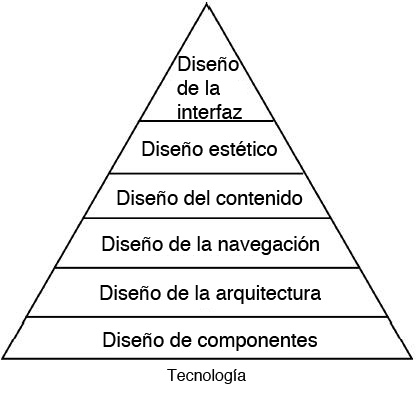
\includegraphics[width=6cm]{img/jpg/piramide.jpg}
		     \caption{Pirámide del diseño de la \textit{webapp}.}
		     \label{fig:dis_piramide}
		   \end{figure}
			
			
			El \textbf{diseño del contenido} utiliza el contenido del modelo (desarrollado durante el análisis) como la base para establecer el diseño de los objetos del contenido. El \textbf{diseño estético (también llamado diseño gráfico)} establece la vista y sensación que el usuario final percibe. El \textbf{diseño arquitectónico} se centra en la estructura general de  hipermedios de todos los objetos y funciones del contenido. El \textbf{diseño de la interfaz} establece la distribución y mecanismos de distribución que definen a la interfaz de usuario. El \textbf{diseño de navegación} define la forma en la que el usuario final navega a través de la estructura de hipermedios. Y el \textbf{diseño de los componentes} representa la estructura interna detallada de los elementos funcionales de la \textit{webapp}.
		
		% subsection pasos_a_seguir (end)
	
		%\begin{figure}[H]
		%  \centering
		%    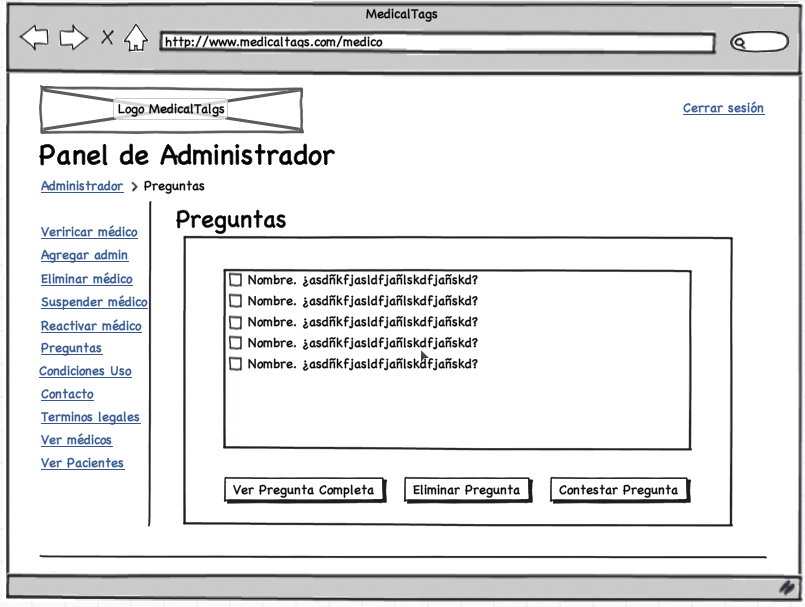
\includegraphics[width=12cm]{img/png/interfaz/99_Administrador.png}
		%  \caption{Panel de Administrador. Preguntas.}
		%  \label{fig:iu_admin_preguntas}
		%\end{figure}
	
	
	% section introduccion (end)
\end{document}
% chapter diseño (end)